\tikzset{
    vert/.style = {
        draw,
        circle,
        inner sep = 1pt,
        minimum size = 10pt
    }
}


    
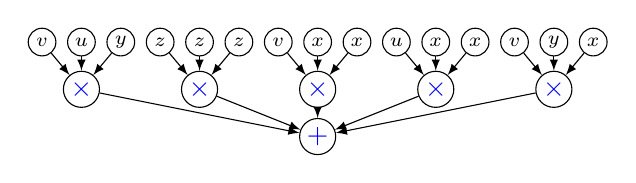
\begin{tikzpicture}[>=latex]
    \pgfmathsetseed{100011}

    \def\vars{{"$x$","$y$","$z$","$u$","$v$","$w$"}}
    
    \node[vert] (a) at (0, 0) {\textcolor{blue}{$+$}};

    \foreach \i in {1, 2, ..., 5}{ 
        \node[vert] (b) at ({1.5 * (\i - 3)}, 0.6) {\textcolor{blue}{$\times$}};
        \foreach \j in {1, 2, 3}{
            \pgfmathsetmacro\inp{int(round(5 * abs(rand)))}
            \node[vert] (c) at ({1.5 * (\i - 3) + 0.5 * (\j - 2)}, 1.2)
                {\scriptsize \pgfmathparse{\vars[\inp]}\pgfmathresult};
            \draw[->] (c) -- (b);
        }
        \draw[->] (b) -- (a);
    }
\end{tikzpicture}